\chapter{Background}
\label{chp:background}
This chapter provides an overview of the theoretical prerequisites on \ac{ML}, \ac{RS} and the field of adversarial examples that were required for solving the main task of this thesis.

\section{Supervised Learning}
\label{sec:supervised}
The majority of problems from the field of \ac{ML} require a parameterized algorithm $f_\theta$ to perform a mapping $f_\theta: X \to Y $, where $ X $ is the input space and $Y$ the output space. For example, in visual recognition, $ X $ might be the space of images, while $ Y $ could be the interval $[0,1]$ describing the probability of a dog appearing in it. Since it is often not trivial to manually specify this function $f$ by traditional means, the supervised learning paradigm offers an alternate approach, which takes advantage of the fact that in many cases, it is relatively easy to acquire a dataset containing examples of the desired mapping. Using these observations, it is possible to train a parametric model, approximating function $f$ iteratively. After successful training, this approximated function can then predict values of $Y$ for unobserved inputs of \(X\)~\parencite{Karpathy:2016}.

In order to find an acceptable approximation, we need an objective function for measuring the disagreement between a model's prediction $\hat{y} = f_\theta(x)$ and the ground truth $y$, i.e., $\mathcal{L}(\hat{y},y) \rightarrow \mathbb{R}$. Such a function is usually known as the \textit{loss} or \textit{error} function and is the primary quality measure used while training a model. A widely used loss function for regression problems is the \ac{MSE}:
\begin{equation}
\mathcal{L}_{MSE}(\hat{y}, y)=\frac{1}{n}\sum_{i=1}^n(\hat{y}_i-y_i)^2\;,
\end{equation}
while in classification tasks, the \ac{CE} loss function is more commonly used and measures the disagreement between two probability distributions, $y$ and $\hat{y}$:
\begin{equation}
\mathcal{L}_{CE}(\hat{y}, y)=-\sum_{k=1}^K(y_k \log \hat{y}_k) = -\log \hat{y}_{y=1}\;.
\end{equation}
Minimizing the task-specific loss function becomes the main objective of the supervised learning task. Usually, a subset of the collected observation is held out for evaluating the model's performance on unseen data. The achieved predictive quality on this test set after training is an indicator of the generalizability of the approximated model $f_\theta$.
\section{Image Classification}
A particularly common supervised learning task is image classification, also known as object recognition. For these types of problems, inputs have the form of 2D pixel intensity matrices in the case of grayscale images and 3D matrices containing separate channel intensities in the case of color images. The channels usually account for the red, green, and blue components of the RGB color space. The outputs are vectors of predicted class probabilities for the given input image, and the goal of the model is to achieve the highest possible accuracy on the test set of unseen images.

Over the years, the research community has established multiple benchmark datasets and competitions for this domain. Beginning with the relatively simple task of handwritten digit recognition, also known as the \ac{MNIST} dataset \parencite{lecun2010mnist}, as seen in Figure~\ref{fig:mnist}, and evolving into more realistic and complex scenarios like the ImageNet challenge \parencite{russakovsky2015imagenet}, also known as the \ac{ILSVRC}, as seen in Figure~\ref{fig:lscrv}, where the dataset contains over 14 million images from over 20,000 classes.
\begin{figure}[H]
	\centering
	\subfloat{
		
\includegraphics[width=0.075\textwidth]{images/mnist/0-0}
	}
	\subfloat{
		
\includegraphics[width=0.075\textwidth]{images/mnist/1-0}
	}
	\subfloat{
		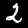
\includegraphics[width=0.075\textwidth]{images/mnist/2-0}
	}
	\subfloat{
		
\includegraphics[width=0.075\textwidth]{images/mnist/3-0}
	}
	\subfloat{
		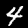
\includegraphics[width=0.075\textwidth]{images/mnist/4-0}
	}
	\subfloat{
		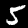
\includegraphics[width=0.075\textwidth]{images/mnist/5-0}
	}
	\subfloat{
		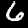
\includegraphics[width=0.075\textwidth]{images/mnist/6-0}
	}
	\subfloat{
		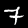
\includegraphics[width=0.075\textwidth]{images/mnist/7-0}
	}
	\subfloat{
		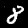
\includegraphics[width=0.075\textwidth]{images/mnist/8-0}
	}
	\subfloat{
		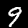
\includegraphics[width=0.075\textwidth]{images/mnist/9-0}
	}\\
	\subfloat{
		
\includegraphics[width=0.075\textwidth]{images/mnist/0-1}
	}
	\subfloat{
		
\includegraphics[width=0.075\textwidth]{images/mnist/1-1}
	}
	\subfloat{
		
\includegraphics[width=0.075\textwidth]{images/mnist/2-1}
	}
	\subfloat{
		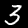
\includegraphics[width=0.075\textwidth]{images/mnist/3-1}
	}
	\subfloat{
		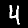
\includegraphics[width=0.075\textwidth]{images/mnist/4-1}
	}
	\subfloat{
		
\includegraphics[width=0.075\textwidth]{images/mnist/5-1}
	}
	\subfloat{
		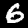
\includegraphics[width=0.075\textwidth]{images/mnist/6-1}
	}
	\subfloat{
		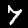
\includegraphics[width=0.075\textwidth]{images/mnist/7-1}
	}
	\subfloat{
		
\includegraphics[width=0.075\textwidth]{images/mnist/8-1}
	}
	\subfloat{
		
\includegraphics[width=0.075\textwidth]{images/mnist/9-1}
	}\\
	\subfloat{
		
\includegraphics[width=0.075\textwidth]{images/mnist/0-2}
	}
	\subfloat{
		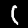
\includegraphics[width=0.075\textwidth]{images/mnist/1-2}
	}
	\subfloat{
		
\includegraphics[width=0.075\textwidth]{images/mnist/2-2}
	}
	\subfloat{
		
\includegraphics[width=0.075\textwidth]{images/mnist/3-2}
	}
	\subfloat{
		
\includegraphics[width=0.075\textwidth]{images/mnist/4-2}
	}
	\subfloat{
		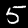
\includegraphics[width=0.075\textwidth]{images/mnist/5-2}
	}
	\subfloat{
		
\includegraphics[width=0.075\textwidth]{images/mnist/6-2}
	}
	\subfloat{
		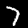
\includegraphics[width=0.075\textwidth]{images/mnist/7-2}
	}
	\subfloat{
		
\includegraphics[width=0.075\textwidth]{images/mnist/8-2}
	}
	\subfloat{
		
\includegraphics[width=0.075\textwidth]{images/mnist/9-2}
	}
	\caption{Randomly sampled images of each class from the \ac{MNIST} digit datset.}
	\label{fig:mnist}
\end{figure}
\begin{figure}[H]
	\centering
	\subfloat[][snail]{
		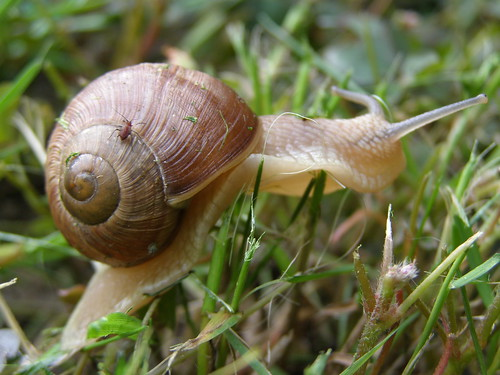
\includegraphics[height=0.15\textwidth]{images/imagenet/snail}
	}
	\subfloat[][bridge]{
		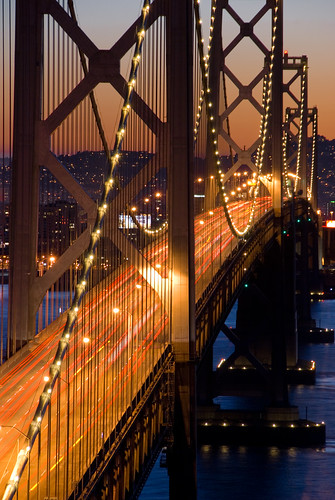
\includegraphics[height=0.15\textwidth]{images/imagenet/bridge}
	}
	\subfloat[][gazania]{
		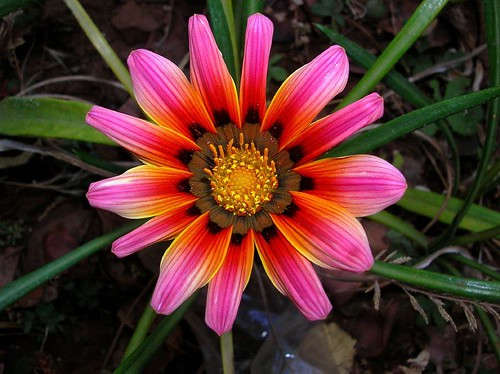
\includegraphics[height=0.15\textwidth]{images/imagenet/gazania}
	}
	\subfloat[][meerkat]{
		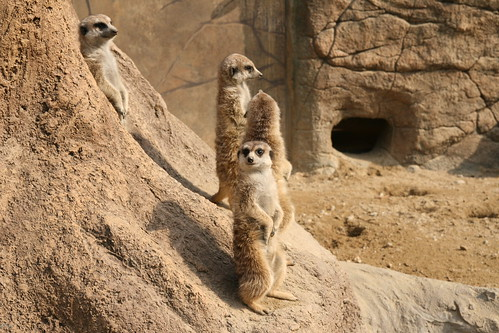
\includegraphics[height=0.15\textwidth]{images/imagenet/meerkat}
	}
	\subfloat[][bok choy]{
		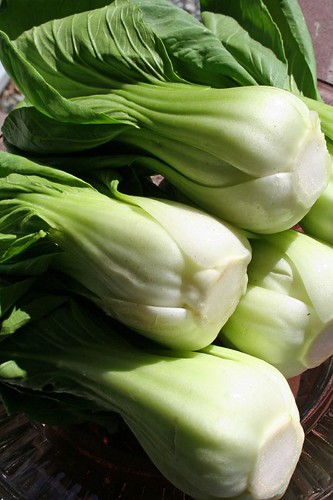
\includegraphics[height=0.15\textwidth]{images/imagenet/bok-choy}
	}\\
	\subfloat[][lobster]{
		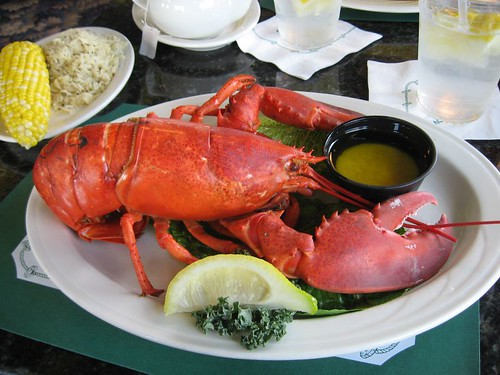
\includegraphics[height=0.15\textwidth]{images/imagenet/lobster}
	}
	\subfloat[][basenji]{
		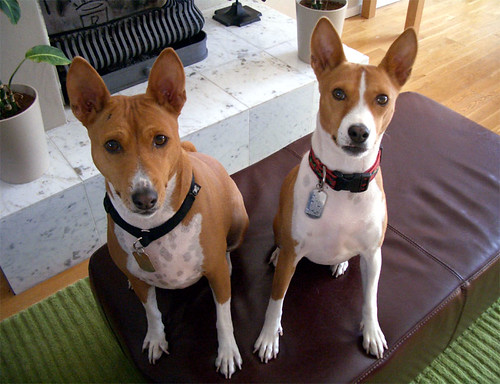
\includegraphics[height=0.15\textwidth]{images/imagenet/basenji}
	}
	\subfloat[][gorilla]{
		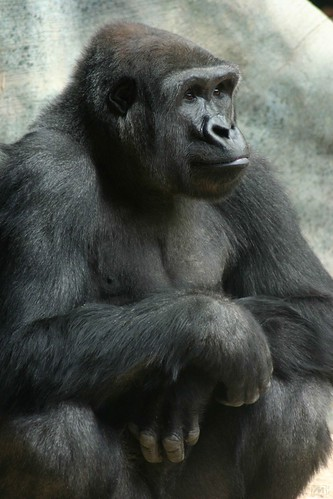
\includegraphics[height=0.15\textwidth]{images/imagenet/gorilla}
	}
	\subfloat[][shark]{
		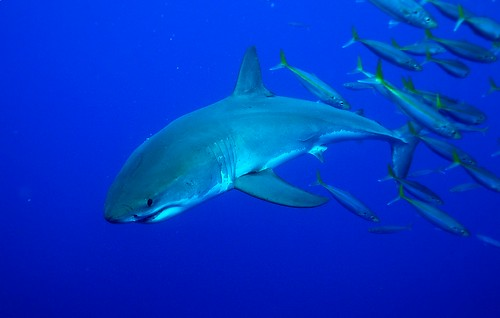
\includegraphics[height=0.15\textwidth]{images/imagenet/shark}
	}
	\subfloat[][piano]{
		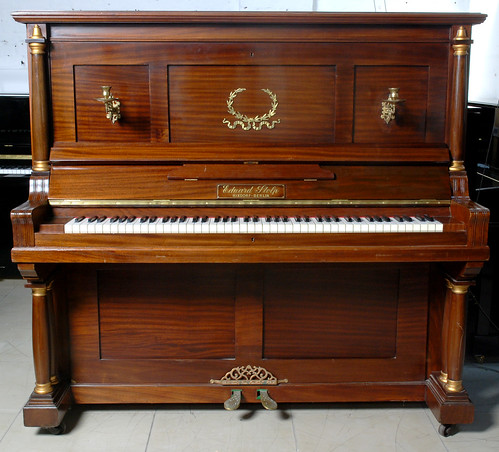
\includegraphics[height=0.15\textwidth]{images/imagenet/piano}
	}
	\caption{Randomly sampled images from the ImageNet challenge.}
	\label{fig:lscrv}
\end{figure}
\section{Optimization}
\label{sec:optimization}
In Section~\ref{sec:supervised}, we introduced the concept of a loss function $\mathcal{L}$, which measures the performance of a prediction. In order to optimize a parameterized model $f_\theta$, we also need an algorithm that can derive a parameter update aimed at minimizing this loss function.

The problem of general optimization is given a function $f: X \to  Y$ to find values $\hat{x}$ that minimizes $f$, i.e., $\hat{x} = \arg \min f(x)$.
To optimize a differentiable function $f$, one commonly used method is called \textit{gradient descent}. Starting at a randomly initialized value for $\hat{x}$, gradients $\frac{\partial f}{\partial \hat{x}}$ are calculated to iteratively adjust the parameters $\hat{x}$ towards the negative direction of the gradients. The gradient is a vector of partial derivatives, representing the slope of the function along each dimension of the parameter space, i.e. given $f(x_1,...,x_n)$ the gradient is defined as $\nabla f = \left(\frac{\partial f}{\partial x_1}, ..., \frac{\partial f}{\partial x_n} \right)^T$. In cases where analytically solving an optimization problem is computationally infeasible, \textit{gradient descent} can be used to iteratively minimize a differentiable function as seen in Figure~\ref{fig:gd}. In the case of optimizing parameterized models using a loss function $\mathcal{L}$, as presented in Section~\ref{sec:supervised}, we calculate the gradients of our loss function in respect to the parameters of the model $\nabla_\theta \mathcal{L}(f_\theta(x_i), y_i)$ and use gradient descent to iterativly optimize our model.
\begin{figure}[H]
	\centering
	\begin{tikzpicture}[samples=50,smooth]
	\clip(-4,-1) rectangle (4,4);
	\path[bend left,name path=arrowcurve] (-2,4) to[out=-30,in=-160] (0,0);
	\foreach \y[count=\i] in {20,16,12,8,4,1,0.0625}{
		\pgfmathsetmacro\colper{\y*4} % color percentage variable
		\draw[name path global/.expanded=curve\i,white!\colper!black] plot[domain=0:360] ({cos(\x)*sqrt(\y/(sin(2*\x)+2))},{sin(\x)*sqrt(\y/(sin(2*\x)+2))});
		\draw[name intersections = {of ={curve\i} and arrowcurve}](intersection-1) coordinate (P\i);
		\ifnum\i=1 
		% do nothing
		\else%
		\pgfmathtruncatemacro\imin{\i-1}
		\pgfmathtruncatemacro\iprint{\i-2}
		\draw[->, color=color1, thick] (P\imin) -- (P\i) node[above right,midway] {$x_\iprint$}; 
		\fi%
	\node {\color{color3}\tiny\faCircle};
	}
\end{tikzpicture}
	\caption{Visualization of the \textit{gradient descent} algorithm where steps are taken following the direction of the slope (negative gradient) at each iteration. Here $x_0$ to $x_5$ represent data points on the contour plot of a loss function whose minimum is at the red dot in the center.}
	\label{fig:gd}
\end{figure}
In practice, datasets can be very extensive, containing millions of training examples. This circumstance makes the exact calculation of gradients across the whole training data, computationally infeasible. Therefore, the gradients are usually estimated using small batches of examples, resulting in a larger amount of approximate parameter updates, instead of fewer exact ones. This method speeds up training and has proven to work well in most practical use cases \parencite{shamir2013stochastic}. Algorithm~\ref{alg:sgd} depicts the individual steps of this procedure.  The described algorithm is called \ac{SGD} and is the basis for most optimizers used for training \acp{DNN}. 
\begin{algorithm}[H]
	\caption{Stochastic Gradient descent (SGD)}
	\label{alg:sgd}
	\begin{algorithmic}[1]
		\Require Training data $\mathcal{D}$;  Learning rate $\eta$;
		\State $\theta \gets$ random parameter initialization
		\Repeat
		\State $(x_i,y_i) \gets$ sample batch from training data $\mathcal{D}$
		\State $\theta \gets \theta - \eta \sum_i \nabla_\theta \mathcal{L}(f_\theta(x_i), y_i)$ \label{alg:sgd:update}
		\Until{convergence}
	\end{algorithmic}
\end{algorithm}
The step size, also known as the learning rate, is a critical parameter for the algorithm. If it is too large, the \ac{SGD} will overshoot local minima, since the slope of the function is constantly changing. Vice versa, if it is too small, a minimum will be found reliably, but the convergence is slow since recalculating the gradients for each step is time-consuming. More advanced variants of \ac{SGD} like AdaGrad~\parencite{Duchi:2011}, Adam~\parencite{Kingma:2014} or RMSProp~\parencite{Hinton:2012} are used in practice to speed up convergence. They achieve this by taking into account previous gradients and momentum while computing the updates for an optimization step (Algorithm~\ref{alg:sgd},~Line~\ref{alg:sgd:update}).
\section{Artificial Neural Networks}
The previous sections described how a parametric model $f_\theta$, consisting of differentiable functions, can be used to transform the inputs $x_i$ to predicted outputs $\hat{y}_i = f_\theta(x_i)$ and how the parameters of such a model can be iteratively optimized using the \ac{SGD} algorithm. This section further details the definition of this function $f_\theta$ for traditional feedforward networks and \acp{CNN}, a particular type of \ac{ANN}, which is especially useful for image processing tasks.
\subsection{Feedforward Neural Network}
\label{sec:feedforward}
A feedforward network is characterized by its unidirectional dataflow, meaning that the graph representing the network contains no cyclic connections. Data enters at the inputs and is transformed through the network layers by repeating matrix multiplications and element-wise non-linearities until reaching the output. Feedforward neural networks usually consist of multiple layers, as seen in Figure~\ref{fig:feedforward}. These layers are made up of computational units that fully connect to their next layer's units. In the context of \acp{ANN} the output of a single hidden neuron or computational unit is referred to as its activation. These activations, as seen in Figure~\ref{fig:neuron}, are calculated using a biased weighted sum of their inputs $x_i$ and apply a nonlinear activation function $\varphi$ to the result, i.e.
\begin{equation}
\hat{y} = f_w(x) = \varphi\left(\sum\limits_{i=0}^{n} x_i w_i + b_i\right)
\label{eq:neuron}
\end{equation}
\begin{figure}[H]
	\centering
	\subfloat[][Visualization of an artifical hidden neuron, computing the result of Eqution~\ref{eq:neuron}.]{
		\resizebox{0.45\textwidth}{!}{\begin{tikzpicture}[
basic/.style={draw,text width=1em,text badly centered},
input/.style={basic,circle, thick},
weights/.style={basic,rectangle, thick},
functions/.style={basic,circle, thick},
]
	\node[functions] (center) {};
	\node[below of=center,font=\scriptsize,text width=4em, text centered] {activation function};
	\draw [gray, thin](0em,0.6em) -- (0em,-0.6em);
	\draw [gray, thin](0.6em,0em) -- (-0.6em,0em);
	\begin{scope}[x=1.25pt,y=3.5pt]
	\draw[thick] (0,0) plot[domain=-4:4] (\x,{tanh(\x)});
	\end{scope}
	\node[right of=center] (right) {};
	\path[draw,->] (center) -- (right);
	\node[functions, left=3em of center] (left) {$\sum$};
	\path[draw,->] (left) -- (center);
	\node[weights, left=2em of left] (2) {$w_2$} -- (2) node[input,left of=2] (l2) {$x_2$};
	\path[draw,->] (l2) -- (2);
	\path[draw,->] (2) -- (left);
	\node[below of=2] (dots) {$\vdots$} -- (dots) node[left of=dots] (ldots) {$\vdots$};
	\node[weights,below of=dots] (n) {$w_n$} -- (n) node[input,left of=n] (ln) {$x_n$};
	\path[draw,->] (ln) -- (n);
	\path[draw,->] (n) -- (left);
	\node[weights,above of=2] (1) {$w_1$} -- (1) node[input,left of=1] (l1) {$x_1$};
	\path[draw,->] (l1) -- (1);
	\path[draw,->] (1) -- (left);
	\node[weights,above of=1] (0) {$b$} -- (0) node[input,left of=0] (l0) {1};
	\path[draw,->] (l0) -- (0);
	\path[draw,->] (0) -- (left);
	\node[below of=ln,font=\scriptsize] {inputs};
	\node[below of=n,font=\scriptsize] {weights};
\end{tikzpicture}}
	}
	\hfill
	\subfloat[][Plots of the three most common nonlinear activation functions used in \acp{ANN}.]{
		\resizebox{0.45\textwidth}{!}{% This file was created by tikzplotlib v0.9.3.
\begin{tikzpicture}

\definecolor{color0}{rgb}{0.917647058823529,0.917647058823529,0.949019607843137}
\definecolor{color1}{rgb}{0.298039215686275,0.447058823529412,0.690196078431373}
\definecolor{color2}{rgb}{0.333333333333333,0.658823529411765,0.407843137254902}
\definecolor{color3}{rgb}{0.768627450980392,0.305882352941176,0.32156862745098}

\begin{axis}[
axis background/.style={fill=color0},
axis line style={white},
legend cell align={left},
legend style={fill opacity=0.8, draw opacity=1, text opacity=1, at={(0.03,0.97)}, anchor=north west, draw=none, fill=color0},
tick align=outside,
tick pos=left,
x grid style={white},
xmajorgrids,
xmin=-4.395, xmax=4.29500000000001,
xtick style={color=white!15!black},
y grid style={white},
ymajorgrids,
ymin=-1, ymax=1,
ytick style={color=white!15!black}
]
\addplot [ultra thick, color1]
table {%
-4 0.0179862099620916
-3.9 0.0198403057340775
-3.8 0.0218812709361305
-3.7 0.0241270214176692
-3.6 0.0265969935768659
-3.5 0.0293122307513563
-3.4 0.0322954646984505
-3.3 0.0355711892726362
-3.2 0.0391657227967644
-3.1 0.0431072549410862
-3 0.0474258731775668
-2.9 0.0521535630784178
-2.8 0.0573241758988688
-2.7 0.0629733560569966
-2.6 0.0691384203433469
-2.5 0.0758581800212436
-2.4 0.0831726964939225
-2.3 0.0911229610148563
-2.2 0.0997504891196853
-2.1 0.109096821195613
-2 0.119202922022118
-1.9 0.130108474362998
-1.8 0.141851064900488
-1.7 0.154465265083535
-1.6 0.167981614866076
-1.5 0.182425523806357
-1.4 0.197816111441419
-1.3 0.214165016957442
-1.2 0.231475216500983
-1.1 0.249739894404883
-0.999999999999997 0.268941421369996
-0.899999999999997 0.289050497374997
-0.799999999999997 0.310025518872388
-0.699999999999997 0.331812227831835
-0.599999999999997 0.354343693774205
-0.499999999999997 0.377540668798146
-0.399999999999997 0.401312339887549
-0.299999999999997 0.425557483188342
-0.199999999999997 0.450166002687523
-0.0999999999999965 0.475020812521061
3.5527136788005e-15 0.500000000000001
0.100000000000003 0.524979187478941
0.200000000000004 0.549833997312479
0.300000000000004 0.57444251681166
0.400000000000004 0.598687660112453
0.500000000000004 0.622459331201855
0.600000000000004 0.645656306225796
0.700000000000005 0.668187772168167
0.800000000000004 0.689974481127613
0.900000000000004 0.710949502625005
1 0.731058578630006
1.1 0.750260105595118
1.2 0.768524783499019
1.3 0.785834983042559
1.4 0.802183888558583
1.50000000000001 0.817574476193645
1.6 0.832018385133925
1.7 0.845534734916466
1.80000000000001 0.858148935099513
1.90000000000001 0.869891525637003
2.00000000000001 0.880797077977883
2.1 0.890903178804388
2.20000000000001 0.900249510880315
2.30000000000001 0.908877038985144
2.40000000000001 0.916827303506078
2.50000000000001 0.924141819978757
2.60000000000001 0.930861579656654
2.70000000000001 0.937026643943004
2.80000000000001 0.942675824101132
2.90000000000001 0.947846436921583
3.00000000000001 0.952574126822433
3.10000000000001 0.956892745058914
3.20000000000001 0.960834277203236
3.30000000000001 0.964428810727364
3.40000000000001 0.96770453530155
3.50000000000001 0.970687769248644
3.60000000000001 0.973403006423134
3.70000000000001 0.975872978582331
3.80000000000001 0.97811872906387
3.90000000000001 0.980159694265923
};
\addlegendentry{σ(x)}
\addplot [ultra thick, color2]
table {%
-4 -0.999329299739067
-3.9 -0.999180865670028
-3.8 -0.998999597785841
-3.7 -0.998778241281131
-3.6 -0.998507942332327
-3.5 -0.998177897611199
-3.4 -0.997774927934279
-3.3 -0.997282960099142
-3.2 -0.996682397839651
-3.1 -0.9959493592219
-3 -0.99505475368673
-2.9 -0.993963167350583
-2.8 -0.992631520201128
-2.7 -0.991007453678118
-2.6 -0.989027402201099
-2.5 -0.98661429815143
-2.4 -0.98367485769368
-2.3 -0.980096396266191
-2.2 -0.975743130031451
-2.1 -0.970451936613454
-2 -0.964027580075817
-1.9 -0.956237458127739
-1.8 -0.946806012846268
-1.7 -0.935409070603099
-1.6 -0.921668554406471
-1.5 -0.905148253644866
-1.4 -0.885351648202262
-1.3 -0.861723159313306
-1.2 -0.833654607012155
-1.1 -0.800499021760629
-0.999999999999997 -0.761594155955764
-0.899999999999997 -0.716297870199023
-0.799999999999997 -0.664036770267847
-0.699999999999997 -0.604367777117162
-0.599999999999997 -0.537049566998033
-0.499999999999997 -0.462117157260007
-0.399999999999997 -0.379948962255222
-0.299999999999997 -0.291312612451588
-0.199999999999997 -0.197375320224901
-0.0999999999999965 -0.0996679946249524
3.5527136788005e-15 3.5527136788005e-15
0.100000000000003 0.099667994624959
0.200000000000004 0.197375320224908
0.300000000000004 0.291312612451595
0.400000000000004 0.379948962255228
0.500000000000004 0.462117157260013
0.600000000000004 0.537049566998038
0.700000000000005 0.604367777117166
0.800000000000004 0.664036770267851
0.900000000000004 0.716297870199026
1 0.761594155955767
1.1 0.800499021760631
1.2 0.833654607012157
1.3 0.861723159313307
1.4 0.885351648202264
1.50000000000001 0.905148253644867
1.6 0.921668554406472
1.7 0.9354090706031
1.80000000000001 0.946806012846269
1.90000000000001 0.95623745812774
2.00000000000001 0.964027580075817
2.1 0.970451936613454
2.20000000000001 0.975743130031452
2.30000000000001 0.980096396266192
2.40000000000001 0.98367485769368
2.50000000000001 0.98661429815143
2.60000000000001 0.989027402201099
2.70000000000001 0.991007453678118
2.80000000000001 0.992631520201128
2.90000000000001 0.993963167350583
3.00000000000001 0.99505475368673
3.10000000000001 0.9959493592219
3.20000000000001 0.996682397839651
3.30000000000001 0.997282960099142
3.40000000000001 0.997774927934279
3.50000000000001 0.998177897611199
3.60000000000001 0.998507942332327
3.70000000000001 0.998778241281131
3.80000000000001 0.998999597785841
3.90000000000001 0.999180865670028
};
\addlegendentry{tanh(x)}
\addplot [ultra thick, color3]
table {%
-4 0
-3.9 0
-3.8 0
-3.7 0
-3.6 0
-3.5 0
-3.4 0
-3.3 0
-3.2 0
-3.1 0
-3 0
-2.9 0
-2.8 0
-2.7 0
-2.6 0
-2.5 0
-2.4 0
-2.3 0
-2.2 0
-2.1 0
-2 0
-1.9 0
-1.8 0
-1.7 0
-1.6 0
-1.5 0
-1.4 0
-1.3 0
-1.2 0
-1.1 0
-0.999999999999997 0
-0.899999999999997 0
-0.799999999999997 0
-0.699999999999997 0
-0.599999999999997 0
-0.499999999999997 0
-0.399999999999997 0
-0.299999999999997 0
-0.199999999999997 0
-0.0999999999999965 0
3.5527136788005e-15 3.5527136788005e-15
0.100000000000003 0.100000000000003
0.200000000000004 0.200000000000004
0.300000000000004 0.300000000000004
0.400000000000004 0.400000000000004
0.500000000000004 0.500000000000004
0.600000000000004 0.600000000000004
0.700000000000005 0.700000000000005
0.800000000000004 0.800000000000004
0.900000000000004 0.900000000000004
1 1
1.1 1.1
1.2 1.2
1.3 1.3
1.4 1.4
1.50000000000001 1.50000000000001
1.6 1.6
1.7 1.7
1.80000000000001 1.80000000000001
1.90000000000001 1.90000000000001
2.00000000000001 2.00000000000001
2.1 2.1
2.20000000000001 2.20000000000001
2.30000000000001 2.30000000000001
2.40000000000001 2.40000000000001
2.50000000000001 2.50000000000001
2.60000000000001 2.60000000000001
2.70000000000001 2.70000000000001
2.80000000000001 2.80000000000001
2.90000000000001 2.90000000000001
3.00000000000001 3.00000000000001
3.10000000000001 3.10000000000001
3.20000000000001 3.20000000000001
3.30000000000001 3.30000000000001
3.40000000000001 3.40000000000001
3.50000000000001 3.50000000000001
3.60000000000001 3.60000000000001
3.70000000000001 3.70000000000001
3.80000000000001 3.80000000000001
3.90000000000001 3.90000000000001
};
\addlegendentry{ReLu(x)}
\end{axis}

\end{tikzpicture}
}
	}
	\caption{The anatomy of an artificial hidden neuron}
	\label{fig:neuron}
\end{figure}
\cite{Hornik:1989} first demonstrated that feedforward networks with a sufficiently large amount of hidden units can be considered universal function approximators. Since then, researchers have applied these types of \acp{ANN} successfully to a wide range of real-world tasks, such as \ac{OCR}~\parencite{LeCun:1989} and speech recognition~\parencite{Morgan:1990}. Invented in the 1980s, they are the oldest types of neural networks and have been the basis for more complex architectures such as \acp{CNN} and \acp{RNN}.
\begin{figure}[H]
	\centering
	\def\layersep{1.5cm}
\begin{tikzpicture}[
	shorten >=1pt,->,
	draw=black!50,
	font=\scriptsize,
	node distance=\layersep,
	every pin edge/.style={<-,shorten <=1pt},
	neuron/.style={circle,minimum size=17pt,inner sep=0pt},
	input neuron/.style={neuron, fill=color2!50, draw=color2, thick},
	output neuron/.style={neuron, fill=color3!50, draw=color3, thick},
	hidden neuron/.style={neuron, fill=color1!50, draw=color1, thick},
	annot/.style={text width=4em, text centered}
	]
	
	% Draw the input layer nodes
	\foreach \name / \y in {1,...,3}
	% This is the same as writing \foreach \name / \y in {1/1,2/2,3/3,4/4}
	\node[input neuron, pin={[pin edge={<-}]left:$x_\name$},] (I-\name) at (0,-\y) {};
	
	% set number of hidden layers
	\newcommand\Nhidden{3}
	
	% Draw the hidden layer nodes
	\foreach \N in {1,...,\Nhidden} {
		\foreach \y in {1,...,4} {
			\path[yshift=0.5cm]
			node[hidden neuron] (H\N-\y) at (\N*\layersep,-\y cm) {};
		}
		\node[annot,above of=H\N-1, node distance=1cm] (hl\N) {Hidden layer \N};
	}
	
	% Draw the output layer node
	\node[output neuron,pin={[pin edge={->}]right:$y$}, right= of $(H3-2)!0.5!(H3-3)$] (O) {};
	
	% Connect every node in the input layer with every node in the
	% hidden layer.
	\foreach \source in {1,...,3}
	\foreach \dest in {1,...,4}
	\path (I-\source) edge (H1-\dest);
	
	% connect all hidden stuff
	\foreach [remember=\N as \lastN (initially 1)] \N in {2,...,\Nhidden}
	\foreach \source in {1,...,4}
	\foreach \dest in {1,...,4}
	\path (H\lastN-\source) edge (H\N-\dest);
	
	% Connect every node in the hidden layer with the output layer
	\foreach \source in {1,...,4}
	\path (H\Nhidden-\source) edge (O);
	
	% Annotate the layers
	
	\node[annot,left of=hl1] {Input layer};
	\node[annot,right of=hl\Nhidden] {Output layer};
\end{tikzpicture}
	\caption{Graph for a multilayer \ac{ANN}, containing three hidden layers. All nodes of each layer are fully connected to the next layer.}
	\label{fig:feedforward}
\end{figure}
\subsection{Convolutional Neural Networks}
Convolutional neural networks (\acp{CNN}), also known as ConvNets, first introduced by \cite{LeCun:1989}, are a specialized kind of neural network for processing data with a known grid-like spatial topology (e.g., images, videos, sound spectrograms, character sequences or 3D voxel data). In each of these cases, an input example  $x$ is a multi-dimensional array (tensor). E.g. a $256\times256$ color image is a $256\times256\times3$ tensor (for 3 color channels red, green, blue).  In many of these cases, the input dimensionality is high (e.g., the image above will have approximately 200,000 numbers), and it is therefore infeasible (in both the number of parameters and processing time) to use fully-connected layers as we saw in Section \ref{sec:feedforward}. In these cases, we prefer to design neural network architectures that take advantage of the spatial input topology by using specific local connectivities and reasonable parameter sharing schemes.

The convolutional operation,  the core computational building block  that gave \acp{CNN} their name, provides a solution to this problem. A convolution is a specialized kind of linear operation, and \acp{CNN} are neural networks that use convolution in place of general matrix multiplication in at least one of their layers \parencite{Goodfellow:2016}.

ConvNets are a sequence of layers, and every layer of a ConvNet transforms one volume of activations to another through a differentiable function. We use three main types of layers to build ConvNet architectures -- convolutional, pooling, and fully connected, as already seen in traditional feedforward networks from Section \ref{sec:feedforward}. We will stack these layer types to form a full ConvNet architecture. In the following sections, we will take a closer look at these unique layer types and their modes of operation.
\subsubsection{Convolutional Layer}
In the general case, a discrete convolution operation implements the function:
\begin{equation}
s(i)=\sum_{a=-\inf}^{\inf}x(a)k(i-a)
\label{eq:conv1}
\end{equation}
where $x$ is the input and $k$ a weighting function known as a kernel. In the case of image processing \acp{CNN}, the input $I$, as well as the kernels $K$, also known as filters, are typically two-dimensional so that we can write out  the convolution function with both axes $(i,j)$ as \parencite{stanford2020cs231n}:
\begin{equation}
S(i,j)=\sum_{m}\sum_{n}I(m,n)K(i-m,j-n)
\label{eq:conv2}
\end{equation}
The convolutional layer’s learnable parameters consist of a set of filters. During the forward pass, we slide (more precisely, convolve) each filter across the width and height of the input volume and compute dot products between the entries of the filter and the input at any position. As we slide the filter over the width and height of the input volume, we will produce a 2-dimensional activation map that gives the responses of that filter at every spatial position. We can visualize this procedure, as seen in Figure \ref{fig:conv}.
\begin{figure}[H]
	\centering
	\resizebox{0.6\textwidth}{!}{\begin{tikzpicture}

	\matrix (mtr) [matrix of nodes,row sep=-\pgflinewidth, nodes={draw}]
	{
		0 & 1 & 1 & |[fill=color3!30]| 1 & |[fill=color3!30]| 0 & |[fill=color3!30]| 0 \\
		0 & 0 & 1 & |[fill=color3!30]| 1 & |[fill=color3!30]| 1 & |[fill=color3!30]| 0 \\
		0 & 0 & 0 & |[fill=color3!30]| 1 & |[fill=color3!30]| 1 & |[fill=color3!30]| 1 \\
		0 & 0 & 0 & 1 & 1 & 0 \\
		0 & 0 & 1 & 1 & 0 & 0 \\
		0 & 1 & 1 & 0 & 0 & 0 \\
	};
	\node[below = 0em of mtr] (lm) {\scriptsize $I$};
	\node[right = 0.2em of mtr] (str) {$*$};
	
	\matrix (K) [right=0.2em of str,matrix of nodes,row sep=-\pgflinewidth, nodes={draw, fill=color1!10}]
	{
		1 & 0 & 1 \\
		0 & 1 & 0 \\
		1 & 0 & 1 \\
	};

	\node[anchor=south east, inner sep=0.01em, color1] at (mtr-1-4.south east) (xx) {\scalebox{.5}{$\times 1$}};
	\node[anchor=south east, inner sep=0.01em, color1] at (mtr-1-5.south east) (xx) {\scalebox{.5}{$\times 0$}};
	\node[anchor=south east, inner sep=0.01em, color1] at (mtr-1-6.south east) (xx) {\scalebox{.5}{$\times 1$}};
	\node[anchor=south east, inner sep=0.01em, color1] at (mtr-2-4.south east) (xx) {\scalebox{.5}{$\times 0$}};
	\node[anchor=south east, inner sep=0.01em, color1] at (mtr-2-5.south east) (xx) {\scalebox{.5}{$\times 1$}};
	\node[anchor=south east, inner sep=0.01em, color1] at (mtr-2-6.south east) (xx) {\scalebox{.5}{$\times 0$}};
	\node[anchor=south east, inner sep=0.01em, color1] at (mtr-3-4.south east) (xx) {\scalebox{.5}{$\times 1$}};
	\node[anchor=south east, inner sep=0.01em, color1] at (mtr-3-5.south east) (xx) {\scalebox{.5}{$\times 0$}};
	\node[anchor=south east, inner sep=0.01em, color1] at (mtr-3-6.south east) (xx) {\scalebox{.5}{$\times 1$}};

	\node[below = 0em of K] (lk) {\scriptsize $K$};
	\node[right = 0.2em of K] (eq) {$=$};

	\matrix (ret) [right=0.2em of eq,matrix of nodes,row sep=-\pgflinewidth, nodes={draw}]
	{
		1 & 4 & 3 & |[fill=color2!30]| 4 \\
		1 & 2 & 4 & 3 \\
		1 & 2 & 3 & 4 \\
		1 & 3 & 3 & 1 \\
	};

	\node[below = 0em of ret] (lim) {\scriptsize $I * K$};

	\draw[very thick, color3] (mtr-1-4.north west) rectangle (mtr-3-6.south east);
	\draw[very thick, color1] (K-1-1.north west) rectangle (K-3-3.south east);
	\draw[very thick, color2] (ret-1-4.north west) rectangle (ret-1-4.south east);

	\draw[densely dotted, color1, thick] (mtr-1-4.north west) -- (K-1-1.north west);
	\draw[densely dotted, color1, thick] (mtr-3-4.south west) -- (K-3-1.south west);
	\draw[densely dotted, color1, thick] (mtr-1-6.north east) -- (K-1-3.north east);
	\draw[densely dotted, color1, thick] (mtr-3-6.south east) -- (K-3-3.south east);
	
	\draw[densely dotted, color2, thick] (ret-1-4.north west) -- (K-1-1.north west);
	\draw[densely dotted, color2, thick] (ret-1-4.south west) -- (K-3-1.south west);
	\draw[densely dotted, color2, thick] (ret-1-4.north east) -- (K-1-3.north east);
	\draw[densely dotted, color2, thick] (ret-1-4.south east) -- (K-3-3.south east);


\end{tikzpicture}}
	\caption{A diagram expressing a two-dimensional convolutional operator as an operation of sliding the kernel matrix $K$ across the target image $I$ and recording elementwise products.}
	\label{fig:conv}
\end{figure}
\subsubsection{Pooling Layer}
To further control the computational complexity and achieve invariance to small translations of the input, it is common practice to use pooling layers to decrease the representation with a fixed downsampling transformation (i.e., without any learnable parameters). In particular, the pooling layers operate on each activation map independently and downsample them spatially \parencite{Karpathy:2016}.  Two commonly used pooling operations are mean-pooling and max-pooling. The mean-pooling operation is defined as:
\begin{equation}
\frac{1}{|u||v|}\sum_{i\in u}\sum_{j\in v}I(i,j)
\label{eq:meanpooling}
\end{equation}
while the max-pooling operation is defined as:
\begin{equation}
\max_{i\in u, j \in v} I(i, j).
\label{eq:maxpooling}
\end{equation}
In both cases, $u$, $v$ are vectors of kernel indices and a visual representation of both pooling operations is provided in Figure \ref{fig:pooling}.
\begin{figure}[H]
	\centering
	\subfloat[][Visualization of the \textit{mean pooling} operation. Color coded patches are combined via arithmetic average.]{
		\resizebox{0.45\textwidth}{!}{\begin{tikzpicture}

\matrix (in) [matrix of nodes,row sep=-\pgflinewidth, nodes={draw}]
{
	|[fill=color1!30]| 4 & |[fill=color1!30]| 7 & |[fill=color2!30]| 1 & |[fill=color2!30]|3\\
	|[fill=color1!30]| 3 & |[fill=color1!30]| 6 & |[fill=color2!30]| 0 & |[fill=color2!30]|8\\
	|[fill=color3!30]| 9 & |[fill=color3!30]| 2 & |[fill=color5!30]| 6 & |[fill=color5!30]|1\\
	|[fill=color3!30]| 1 & |[fill=color3!30]| 4 & |[fill=color5!30]| 1 & |[fill=color5!30]|0\\
};

\node [below=0em of in] (lin) {\tiny Input};

\matrix (out) [matrix of nodes,row sep=-\pgflinewidth, nodes={draw}, right=4em of in]
{
	|[fill=color1!30]| 5 & |[fill=color2!30]| 3 \\
	|[fill=color3!30]| 4 & |[fill=color5!30]| 2 \\
};

\node [below=0em of out] (lout) {\tiny Output};

\draw[->] (in) to node[above]{\scriptsize Mean} node[below]{\scriptsize Pooling} (out);

\draw[very thick, color1] (in-1-1.north west) rectangle ($(in-2-2.south east) + (0,0.4pt)$);
\draw[very thick, color2] (in-1-4.north east) rectangle ($(in-2-3.south west) + (0,0.4pt)$);
\draw[very thick, color3] (in-4-2.south east) rectangle (in-3-1.north west);
\draw[very thick, color5] (in-4-4.south east) rectangle (in-3-3.north west);

\draw[very thick, color1] (out-1-1.north west) rectangle ($(out-1-1.south east) + (0,0.4pt)$);
\draw[very thick, color2] (out-1-2.north east) rectangle ($(out-1-2.south west) + (0,0.4pt)$);
\draw[very thick, color3] (out-2-1.north west) rectangle (out-2-1.south east);
\draw[very thick, color5] (out-2-2.north west) rectangle (out-2-2.south east);

\end{tikzpicture}}
	}
	\hfill
	\subfloat[][Visualization of the \textit{max pooling} operation. Color coded patches are downsampled by taking the maximum value found in the patch.]{
		\resizebox{0.45\textwidth}{!}{\begin{tikzpicture}

\matrix (in) [matrix of nodes,row sep=-\pgflinewidth, nodes={draw}]
{
	|[fill=color1!30]| 4 & |[fill=color1!30]| 7 & |[fill=color2!30]| 1 & |[fill=color2!30]|3\\
	|[fill=color1!30]| 3 & |[fill=color1!30]| 6 & |[fill=color2!30]| 0 & |[fill=color2!30]|8\\
	|[fill=color3!30]| 9 & |[fill=color3!30]| 2 & |[fill=color5!30]| 6 & |[fill=color5!30]|1\\
	|[fill=color3!30]| 1 & |[fill=color3!30]| 4 & |[fill=color5!30]| 1 & |[fill=color5!30]|0\\
};

\node [below=0em of in] (lin) {\tiny Input};

\matrix (out) [matrix of nodes,row sep=-\pgflinewidth, nodes={draw}, right=4em of in]
{
	|[fill=color1!30]| 7 & |[fill=color2!30]| 8 \\
	|[fill=color3!30]| 9 & |[fill=color5!30]| 6 \\
};

\node [below=0em of out] (lout) {\tiny Output};

\draw[->] (in) to node[above]{\scriptsize Max} node[below]{\scriptsize Pooling} (out);

\draw[very thick, color1] (in-1-1.north west) rectangle ($(in-2-2.south east) + (0,0.4pt)$);
\draw[very thick, color2] (in-1-4.north east) rectangle ($(in-2-3.south west) + (0,0.4pt)$);
\draw[very thick, color3] (in-4-2.south east) rectangle (in-3-1.north west);
\draw[very thick, color5] (in-4-4.south east) rectangle (in-3-3.north west);

\draw[very thick, color1] (out-1-1.north west) rectangle ($(out-1-1.south east) + (0,0.4pt)$);
\draw[very thick, color2] (out-1-2.north east) rectangle ($(out-1-2.south west) + (0,0.4pt)$);
\draw[very thick, color3] (out-2-1.north west) rectangle (out-2-1.south east);
\draw[very thick, color5] (out-2-2.north west) rectangle (out-2-2.south east);

\end{tikzpicture}}
	}
	\caption{Common pooling operations used in \acp{CNN}.}
	\label{fig:pooling}
\end{figure}

\subsubsection{ConvNet Architectures}
We have seen that \acp{CNN} are commonly made up of only three layer types: convolutional (\texttt{CONV}), pooling (\texttt{POOL}), and fully-connected (\texttt{FC}). We will also explicitly write the activation function as a layer (e.g., \texttt{RELU}), which applies an elementwise non-linearity. In this section, we discuss how these layers are commonly stacked together to form entire ConvNets and which architectures have achieved state-of-the-art performance on the ImageNet challenge.

The most common form of a ConvNet architecture stacks a few \texttt{CONV-RELU} layers, follows them with \texttt{POOL} layers and repeats this pattern until the image has been merged spatially to a small size. At some point, it is common to transition to fully-connected layers. The last fully-connected layer holds the output, such as the class scores. In other words, the most common ConvNet architecture follows the pattern:

\texttt{INPUT -> [[CONV -> RELU]*N -> POOL?]*M -> [FC -> RELU]*K -> FC}

where the \texttt{*} indicates repetition, and the \texttt{POOL?} indicates an optional pooling layer. Additionally, \texttt{N >= 0} (and usually \texttt{N <= 3}), \texttt{M >= 0}, \texttt{K >= 0} (and usually \texttt{K < 3}). 

\acp{CNN} have been successfully applied to image classification tasks. They were first used by \cite{LeCun:1989} to recognize digits from the MNIST dataset and were then widely popularized when \cite{krizhevsky2012imagenet} won the \ac{ILSVRC} 2012 by a large margin with their \ac{CNN} architecture known as AlexNet. Subsequent editions of the challenge were also won by \acp{CNN} like GoogLeNet \parencite{szegedy2015going} or ResNet \parencite{he2016deep}. 

The runner-up in \ac{ILSVRC} 2014 was the network from \cite{simonyan2014very} that became known as VGGNet. Its main contribution was in showing that the depth of the network is critical for good performance. Their final best network, known as VGG-16, visualized in \ref{fig:vgg}, contains 16 \texttt{CONV/FC} layers and features an extremely homogeneous architecture that only performs $3\times3$ convolutions and $2\times2$ pooling from the beginning to the end \parencite{stanford2020cs231n}. 
\begin{figure}[H]
	\centering
	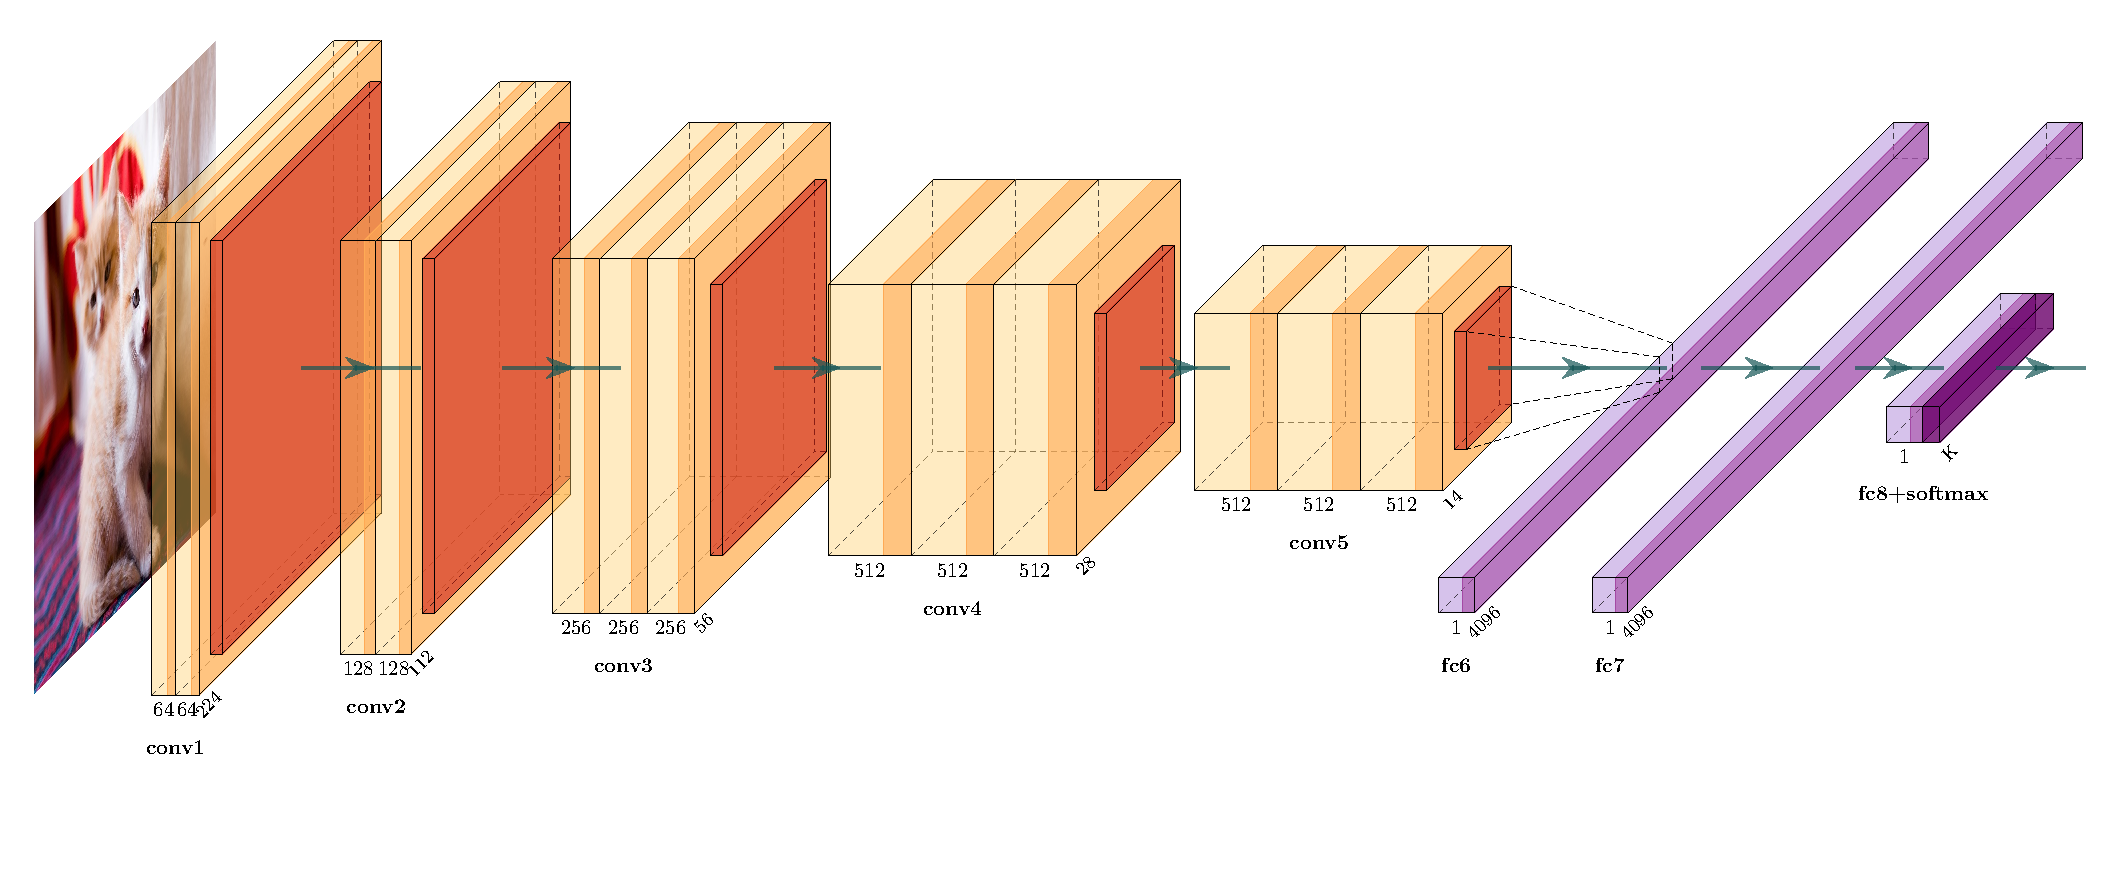
\includegraphics[width=\textwidth]{images/vgg16}
	\caption{Diagram of the  \ac{CNN} architecture of VGG-16}
	\label{fig:vgg}
\end{figure}

\section{Backpropagation}
\label{sec:backprop}
The generic approach of applying \ac{SGD} to compositional models, such as \acp{ANN}, is called backpropagation. Due to the composite form, we can calculate the gradients using the chain rule for differentiation~\parencite[p.~395]{Hastie:2009}.  For a better intuition as to why this is possible, we can look at the functions that the \ac{ANN} in Figure~\ref{fig:backprop} consists of: 
\begin{align}	
h_i&=\varphi\left(\sum\limits_{j=0}^{n} x_j  w_{h_i}^{x_j}\right)\;, \\
\hat{y}&=\sum\limits_{i=0}^{m}h_i w_{\hat{y}}^{h_i}\;, 
\end{align}
where $\varphi$ is a differentiable activation function, $n$ represents the number of inputs, $m$ equals the number of hidden neurons, $x_j$ refers to the inputs and $w_x^y$ are the weights in neuron $x$ for input $y$.

The partial derivative of the loss function $\mathcal{L}$, with respect to a weight $w_{h_i}^{x_j}$ in a hidden neuron $h_i$ for input $x_j$, results from applying the chain rule
\begin{equation}
\frac{\partial \mathcal{L}}{\partial w_{h_i}^{x_j}} = \frac{\partial \mathcal{L}}{\partial \hat{y}} \frac{\partial \hat{y}}{\partial \mbox{h}_{i}} \frac{\partial \mbox{h}_{i}}{\partial w_{h_i}^{x_j}}\;.
\end{equation}
The resulting value indicates, in which direction the respective weight $w_{h_i}^{x_j}$ has to be adjusted by an infinitesimally small amount, in order to decrease the loss $\mathcal{L}$~\parencite[p.~169]{Rojas:2013}. For simplicity reasons, the bias of each neuron is omitted.

\begin{figure}
	\centering
	\begin{tikzpicture}[
shorten >=1pt,->,
font=\scriptsize,
node distance=0.75cm and 1.75cm,
every pin edge/.style={<-,shorten <=1pt},
neuron/.style={circle,minimum size=20pt,inner sep=0pt},
input neuron/.style={neuron, fill=color2!50, draw=color2, thick},
output neuron/.style={neuron, fill=color3!50, draw=color3, thick},
hidden neuron/.style={neuron, fill=color1!50, draw=color1, thick},
activation/.style={draw=color2!75!black!50, thick, bend angle=15},
gradient/.style={draw=color3!75!black!50, thick, bend angle=45},
]

\node[input neuron] (x0) {$x_0$};
\node[input neuron, below=of x0] (x1) {$x_1$};
\node[input neuron, below=of x1] (x2) {$x_2$};

\node[hidden neuron, right=of $(x0)!0.5!(x1)$] (h0) {$h_0$};
\node[hidden neuron, right=of $(x1)!0.5!(x2)$] (h1) {$h_1$};

\node[output neuron, right=of $(h0)!0.5!(h1)$] (y) {$\hat{y}$};

\draw[activation, ->, bend left] (x0) to node[above, sloped]{\color{color2}$activations$} (h0);
\draw[activation, ->, bend right] (x0) to (h1);
\draw[activation, ->, bend left] (x1) to (h0);
\draw[activation, ->, bend right] (x1) to (h1);
\draw[activation, ->, bend left] (x2) to (h0);
\draw[activation, ->, bend right] (x2) to (h1);

\draw[activation, ->, bend right] (h0) to (y);
\draw[activation, ->, bend left] (h1) to (y);

\draw[gradient, ->, bend right] (y) to node[above, sloped]{\color{color3}$gradients$} (h0);
\draw[gradient, ->, bend left] (y) to (h1);

\end{tikzpicture}
	\caption{Backpropagation in a single hidden layer \ac{ANN}. After a set of inputs is processed in the forward pass (green), the final error is determined and the gradients (contribution of neurons to error) are calculated recursively using the chain rule in the backward pass (red).}
	\label{fig:backprop}
\end{figure}


\subsection{Numerical Example} 
In order to further illustrate the process of backpropagation, a complete forward and partial backward pass of the \ac{ANN} in Figure~\ref{fig:backprop} is conducted.

Using a \ac{ReLU} as an activation function:
\begin{equation}
\varphi(x) = max(0,x)
\end{equation}

\textbf{Note.} \ac{ReLU} is technically not differentiable at $x=0$, but is still widely used, due to its empirical performance. It is common practice to set the derivative at this discontinuity to zero or one~\parencite[p.~4]{Nair:2010}.

Given inputs $x_i$ and a label $y$:
\begin{align}
x_0 &= 0 & x_1 &= 1 & x_2 &= 0 & y &= 1
\end{align}

Weights for all hidden and output neurons:
\begin{align}
w_{h_0}^{x_0} &= 0.0 & w_{h_0}^{x_1} &= 0.1 & w_{h_0}^{x_2} &= 0.2 \\
w_{h_1}^{x_0} &= 0.2 & w_{h_1}^{x_1} &= 0.4 & w_{h_1}^{x_2} &= 0.6 \notag\\
w_{\hat{y}}^{h_0} &= 0.3& w_{\hat{y}}^{h_1} &= 0.2 \notag
\end{align}

Activation of the first hidden neuron $h_0$:
\begin{align}
h_0 &=\varphi(x_0 w_{h_0}^{x_0} + x_1 w_{h_0}^{x_1} + x_2 w_{h_0}^{x_2})\\
&= \max(0,\,0\cdot0.0+1\cdot0.1+0\cdot0.2) \notag\\
&= 0.1 \notag
\end{align}

Activation of the second hidden neuron $h_1$:
\begin{align}
h_1 &= \varphi(x_0 w_{h_1}^{x_0} + x_1 w_{h_1}^{x_1} + x_2 w_{h_1}^{x_2})\\
&= \max(0,\,0\cdot0.2+1\cdot0.4+0\cdot0.6) \notag\\
&= 0.4 \notag
\end{align}

Activation of the output neuron $\hat{y}$:
\begin{align}
\hat{y} &= h_0 w_{\hat{y}}^{h_0} + h_1 w_{\hat{y}}^{h_1} \\
&= 0.1\cdot0.3 + 0.4\cdot0.2 \notag\\
&= 0.11 \notag
\end{align}

The squared error loss $\mathcal{L}$ is calculated with respect to expected label $y$:
\begin{equation}
\mathcal{L} = (\hat{y}-y)^2 = (0.11-1)^2 = 0.7921
\end{equation}

Since $\mathcal{L}$ is a composite function of $\hat{y}$ (which in turn is again a composite function of $h_1$ and $h_0$), the chain rule of differentiation has to be applied, in order to compute the gradients of $\frac{\partial \mathcal{L}}{\partial w_{\hat{y}}^{h_0}}$ and $\frac{\partial \mathcal{L}}{\partial w_{\hat{y}}^{h_1}}$:
\begin{align}
\frac{\partial \mathcal{L}}{\partial w_{\hat{y}}^{h_0}} &= \frac{\partial \mathcal{L}}{\partial \hat{y}}\frac{\partial \hat{y}}{\partial w_{\hat{y}}^{h_0}} = 2(\hat{y}-y) \cdot h_0 = -0.178\\
\frac{\partial \mathcal{L}}{\partial w_{\hat{y}}^{h_1}} &= \frac{\partial \mathcal{L}}{\partial \hat{y}}\frac{\partial \hat{y}}{\partial w_{\hat{y}}^{h_1}} = 2(\hat{y}-y) \cdot h_1 = -0.712
\end{align}

The resulting gradients indicate the sensitivity of $\mathcal{L}$ for $w_{\hat{y}}^{h_0}$ and $w_{\hat{y}}^{h_1}$.
In other words how much $\mathcal{L}$ would change if $w_{\hat{y}}^{h_0}$ or $w_{\hat{y}}^{h_1}$ were adjusted. For a complete backward pass, the gradients for all weights of $h_1$ and $h_0$ would be calculated, by further chaining the partial derivatives. Assuming the optimizer algorithm is \ac{SGD}, the results would be multiplied by an infinitesimally small $learning\,rate$ and subtracted from the respective weights during an update step, resulting in a slightly lower value of $\mathcal{L}$.

\subsection{Computational Graph}
It is often more intuitive to think of the functions that make up an \ac{ANN}, as a \ac{DAG}, instead of a linear sequence of operations. Vectors flow along the edges of this graph and nodes perform differentiable transformation on these vectors. Most implementations of backpropagation use some kind of graph representation that keeps track of all nodes and operations inside this graph.

The graph and nodes both implement a \texttt{forward()} and \texttt{backward()} operation. 
During the \texttt{forward()} pass, the graph calls all nodes' \texttt{forward()} operations in the correct topological order, each time supplying the outputs of the last node as inputs to the next.

The graph's \texttt{backward()} implementation operates in the reverse order, starting with the loss and recursively chaining (multiplying) the nodes' gradients together until the end of the graph is reached.
\textit{PyTorch}---the deep learning framework used in the context of this thesis---also makes use of such graph representation~\parencite{paszke2019pytorch}.
\section{Recommendation Systems}
Recommendation systems (\acp{RS}) are \acp{DSS} which analyze patterns of user behavior to provide them with personalized content recommendations that suit their preference. The main reason for online services to deploy recommendation systems, is to handle the phenomenon of information overload, which many users face in a world of evergrowing options and available content \parencite{bobadilla2013recommender}. 

More formally, \cite{adomavicius2005toward} define the recommendation problem as follows: Let $C$ be the set of all users and let $S$ be the set of all possible items that can be recommended. Let u be a utility function that measures the usefulness of items to the user c, i.e., $u : C \times S \to R$, where $R$ is an ordered set. Then, for each user $c \in C $, we want to choose such items $s' \in S $ that maximizes the user's utility. More formally:
\begin{equation}
\forall_{c \in C}, \quad s'_c = \arg\max_{s \in S} u(c, s).
\end{equation}
Estimating this utility function, which optimizes a particular performance criterion, is the central part of any \ac{RS}. The utility function for items that a user has not interacted with can be estimated in many different ways using methods from machine learning, approximation theory, and various heuristics. \acp{RS} are usually classified according to their approach to utility estimation \parencite{adomavicius2005toward}, as seen in Figure~\ref{fig:recsys}. 
\begin{figure}[H]
	\centering
	\vspace{1em}
	\begin{forest}
for tree={
  draw,
  align=center,
  l sep=0.3cm,
  s sep=0.3cm,
  rounded corners
},
[{Recommendation Systems},
  [{Content-Based}]
  [{Collaborative Filtering}]
  [{Hybrid Approach}]
]
\end{forest}
	\caption{Typical categorization for \acp{RS}.}
	\label{fig:recsys}
\end{figure}
In the following sections, we will review the two main approaches of \ac{CF} and \ac{CBF}, explaining the basic concepts and referencing current state-of-the-art models for both approaches.
\subsection{Collaborative Filtering}
Collaborative Filtering (\acs{CF}) is based on how humans have made decisions throughout history: Besides on our own experiences, we also base our decisions on the experiences and knowledge that reach each of us from a relatively large group of acquaintances \parencite{bobadilla2013recommender}. Therefore \ac{CF} approaches make recommendations to each user based on the either explicit (e.g., ratings) or implicit (e.g., views or purchases) feedback of users who have the most in common with them, as visualized in Figure~\ref{fig:cf}.
\begin{figure}[H]
	\centering
	\begin{tikzpicture}
	\node[alice, scale=2](alice){};
	\node[bob, scale=2, right=of alice, xshift=1cm](bob){};
	
	\node[above=of $(alice)!0.5!(bob)$] (commonDocs) {
		\color{color3}\huge\faFileTextO\,\color{color2}\huge\faFileTextO
	};
	\node[above=of commonDocs, yshift=-1cm] {Viewed by both users};
	
	\node[below=of $(alice)!0.5!(bob)$] (recommendedDoc) {
		\color{color1}\huge\faFileTextO
	};
	\node[below=of recommendedDoc, yshift=1cm, text width=4cm, text centered] {
		Viewed by her,\\recommended to him
	};
	
	\draw[<->, very thick, color1] (alice) to node[above] {Similar users}(bob);
	\draw[->, thick, color5] (alice) to (commonDocs);
	\draw[->, thick, color5] (bob) to (commonDocs);
		
	\draw[->, thick, color5] (alice) to (recommendedDoc);
	\draw[->, thick, color2] (recommendedDoc) to (bob);
\end{tikzpicture}
	\caption{Visualization of the collaborative filtering technique}
	\label{fig:cf}
\end{figure}

Among the various collaborative filtering techniques, \ac{MF} \parencite{he2016fast} is the most popular one. This approach projects users and items into a shared latent space, using a  vector of latent features to represent a user or an item. After that, users' interaction on an item is modeled as the inner product of their latent vectors. Popularized by the Netflix Prize, MF has become the defacto standard approach to latent factor model-based recommendation \parencite{he2017neural}. Recently an increasing number of researchers have shown interest in employing \acp{DNN} for \ac{CF} \acp{RS}. Prominent examples from this direction of research include the Wide \& Deep model from Google \parencite{cheng2016wide}, the \ac{NCF} approach published by \cite{he2017neural} and the DeepFM model by \cite{guo2017deepfm}.

\subsection{Content-Based Filtering}
Content-based filtering (\acs{CBF}) generates recommendations using the content from items intended for the recommendation; therefore, specific content needs to be analyzed, like text, images, or sound. A similarity measure between objects can be established from this analysis serving as the basis for recommending items similar to items that a user has bought, visited, heard, viewed, or ranked positively \parencite{bobadilla2013recommender}. This general approach is visualized in Figure~\ref{fig:cbf}. 
\begin{figure}[H]
	\centering
	\begin{tikzpicture}
	\node[bob, scale=2](bob){};
	
	\node[right=of bob, yshift=-1.5pt] (viewedDoc) {\color{color3}\huge\faFileTextO};
	\node[above=of viewedDoc, yshift=-1cm] {Viewed by user};
	
	\node[below=of viewedDoc] (similarDoc) {\color{color2}\huge\faFileTextO};
	\node[below=of similarDoc, yshift=1cm] {Recommend to user};
	
	\draw[<->, very thick, color1] (viewedDoc) to node[right] {Similar items} (similarDoc);
	\draw[->, thick, color5] (bob) to (viewedDoc);
	\draw[->, thick, color2] (similarDoc) to (bob);
\end{tikzpicture}
	\caption{Visualization of the content-based filtering technique}
	\label{fig:cbf}
\end{figure}
For a \ac{CBF} system to operate, attributes of the items intended for recommendation must be extracted \parencite{bobadilla2013recommender}. Depending on the type of content, the approaches for this extraction step vary:

In the case of processing textual information, classic information retrieval techniques can be used to define such attributes automatically (e.g., term frequency, inverse document frequency, and normalization to page length) \parencite{pazzani2007content}. As recent advances in \ac{NLP} using \acp{DNN} have demonstrated the importance of learning good representations for text \parencite{le2014distributed}, researchers have started to use \acp{DNN} in the context of text-based \acp{RS} \parencite{chen2017joint}, achieving superior results compared to classical methods. 
\pagebreak

For visual \acp{RS}, early attempts have primarily employed annotated tags \parencite{fan2008justclick} or low-level visual features \parencite{su2010efficient}, such as color, texture, and shape, to capture the semantics of images. As a result of the success of \acp{DNN} in the domain of computer vision \parencite{he2016deep}, many recent approaches, like \cite{mcauley2015image}, \cite{he2016vbpr}, \cite{bracher2016fashion}, \cite{kang2017visually}, \cite{shankar2017deep}, and \cite{tuinhof2018image} have now also shifted towards using \acp{DNN} for image-based \acp{RS}. More specifically, they utilize \acp{CNN} as feature extractors for images and integrate these product features into purely content-based or hybrid \acp{RS}.

\section{Adversarial Attacks}
Statistical \ac{ML} and especially, \ac{DL} have become increasingly popular due to their superior performance in many tasks and are deployed in many real-world applications, ranging from image classification~\parencite{krizhevsky2012imagenet, he2016deep} to speech recognition~\parencite{hinton2012deep} and \ac{NLP}~\parencite{devlin2018bert}. Because of these accomplishments, \ac{ML} methods have also become an essential tool in many security-sensitive domains, such as spam filtering~\parencite{guzella2009review}, malware detection~\parencite{sahs2012machine}, and network \acp{IDS}~\parencite{yin2017deep}, where these applications are required to be highly accurate, stable, and reliable, even if underlying data distributions change. These requirements stand in contrast to an attacker's goals, who tries to modify the input data to circumvent these systems. \cite{dalvi2004adversarial} has first demonstrated that machine learning models are often vulnerable to manipulations, causing incorrect classification of adversarial inputs. In particular, neural networks are highly vulnerable to attacks based on small modifications to inputs at prediction time, as first pointed out by \cite{szegedy2013intriguing}. More recent research by \cite{grosse2016adversarial} has also proven the existence of adversarial examples for the problem of malware classification. Apart from the security implications, this phenomenon also demonstrates that current models are not learning the underlying concepts in a robust manner \parencite{madry2017towards}. The following sections will give a definition of adversarial examples, explore different attack methods, discuss the property of transferability and lastly, show what kind of defenses exist.
\subsection{Adversarial Examples}
An adversarial example is a sample of input data that has been modified very slightly in a way that intends to cause a machine learning classifier to misclassify it. In many cases, these modifications can be so subtle that a human observer does not even notice the modification at all, as seen in Figure \ref{fig:adv}, yet the classifier still makes a mistake \parencite{kurakin2016adversarial}.

Currently there is no widely agreed-upon explanation as to why these adversarial examples exist, but rather a variety of explanations were proposed. Some researchers have attributed this phenomenon to the high dimensional nature of the input and parameter space \parencite{goodfellow2014explaining}, while others have attributed it to the presence of non-robust features in the training data \parencite{ilyas2019adversarial}.

\begin{figure}[H]
	\centering
	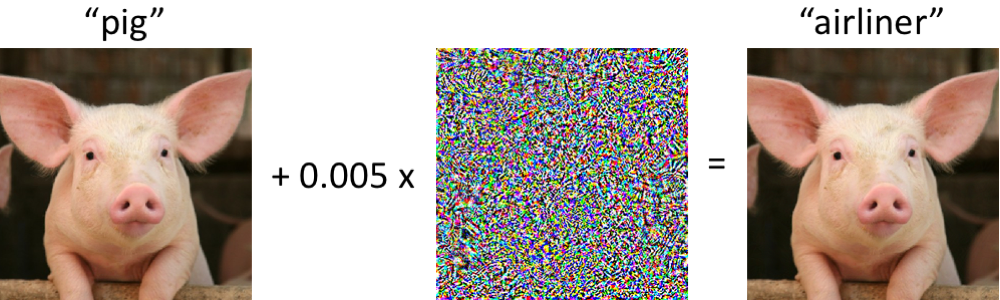
\includegraphics[width=\textwidth]{images/piggie}
	\caption{On the left, we have an image of a pig that is correctly classified as such by a state-of-the-art \ac{CNN}. After perturbing the image slightly (every pixel is in the range [0, 1] and changed by at most 0.005), the network now returns class “airliner” with high confidence \parencite{mit2018adv}.}
	\label{fig:adv}
\end{figure}
More formally \cite{carlini2017towards} defines a targeted adversarial example $x'$ as an example fulfilling the property of $C(x') = t$, where $C$ is a classifier, $x$ an input, $y$ the ground-truth class label and $t\ne y$ the target class, while $x'$ and $x$ are close according to some distance metric. 

A less powerful attack also discussed in the literature instead asks for untargeted adversarial examples:  instead of classifying $x$ as a given target class, we only search for an input $x'$ so that
$C(x')\ne y$ and $x,x'$ are close \parencite{carlini2017towards}.

There  are three widely-used distance metrics in the literature for generating adversarial examples, all of which are $l_p$ norms \parencite{carlini2017towards}.

\begin{enumerate}
	\item $l_0$ distance measures the number of coordinates $i$ such that $x_i \ne x_i' $.
	\item $l_2$ distance measures the standard Euclidean distance between $x$ and $x'$. 
	\item $l_\infty$ distance measures the maximum change to any of the coordinates:
	\begin{equation}
		\|x-x'\|_\infty = \max(|x_1-x'_1|,...,|x_n-x'_n|).
	\end{equation}
\end{enumerate}

\subsection{Finding Adversarial Examples}
The following sections will describe three well-studied white-box attacks and show how they can be used to find targeted adversarial examples. All approaches share a common theme of using the gradients $\nabla_x$ produced by the network with respect to the input for finding adversarial perturbations that optimize for a chosen adversarial goal.

\subsubsection{Fast Gradient Sign Method}
One of the first and most popular adversarial white-box attacks is the single-step \ac{FGSM}, initially described by \cite{goodfellow2014explaining}. Let $x$ be the input to the model, $y$ the label associated with $x$ and $\mathcal{L}(x, y)$ be the loss used to train the model. We can linearize the loss function around the current value of $x$, obtaining an $\epsilon$ constrained perturbation which can be added to the image to obtain an untargeted adversarial example $x'$ that maximizes $\mathcal{L}$, i.e.
\begin{equation}
x' = x + \epsilon\ \text{sign}(\nabla_x\mathcal{L}(x, y)).
\label{eq:fgsm-untargeted}
\end{equation}
In other words, the attack backpropagates the gradient back to the input data to calculate $\nabla_x\mathcal{L}(x, y)$ and then adjusts the input data by a small step $\epsilon$ in the direction that will maximize the loss. 

To use \ac{FGSM} for targeted attacks, trying to maximize the probability for some specific class $t \ne y$, attacking a neural network with \ac{CE} loss will lead to the following formula for the single-step attack \cite{kurakin2016scale}:
\begin{equation}
x' = x - \epsilon\ \text{sign}(\nabla_x\mathcal{L}(x, t)).
\label{eq:fgsm-targeted}
\end{equation}

\subsubsection{Projected Gradient Descent}
A rather simple extension of the original \ac{FGSM} attack is the \ac{PGD} attack, also known as the \ac{BIM}. By iteratively performing the \ac{FGSM} attack with smaller step sizes $\alpha$ and clipping the resulting perturbations after each iteration, more powerful adversarial examples can be found. More formally a untargeted \ac{PGD} attack can be written as \parencite{kurakin2016adversarial}:
\begin{equation}
x'_0 = x,\quad x'_{N+1} = Clip_{x,\epsilon}\Big\{ x'_N + \alpha\ \text{sign}(\nabla_x\mathcal{L}(x'_N, y)) \Big\}.
\label{eq:pgd-untargeted}
\end{equation}
Similar to \ac{FGSM} the targeted version looks very similar:
\begin{equation}
x'_0 = x,\quad x'_{N+1} = Clip_{x,\epsilon}\Big\{ x'_N - \alpha\ \text{sign}(\nabla_x\mathcal{L}(x'_N, t)) \Big\}.
\label{eq:pgd-targeted}
\end{equation}
The exact clipping equation, ensuring valid pixel values ($0\le x' \le 1$) and a maximum $l_\infty$-norm perturbation budget $\epsilon$ for an adversarial example $x'$, is defined as:
\begin{equation}
Clip_{x,\epsilon} \big\{ x' \big\} = \min \Big\{1, x +\epsilon,\max \big\{ 0,x-\epsilon, x'\big\}, \Big\}
\label{eq:clip}
\end{equation}
where $x$ is the channel values of the original image.

\subsubsection{Carlini \& Wagner Method}
The \ac{CW} attack \parencite{carlini2017towards} is one of the most effective white-box attack methods. The core idea of the \ac{CW} attack is to use an unconstrained optimization formulation and an emperically chosen objective function $f$. Formally, for a chosen $l_p$ norm, the problem becomes: given a constant $c$, and an input image $x$, find $\delta$ that solves
\begin{align}
\minimize \quad& \|\delta\|_p + c \cdot f(x+\delta)\\
such\,that \quad& x+ \delta \in[0,1]^n
\label{eq:cw}
\end{align}
To ensure the modification yields a valid image ($0\le x_i+\delta_i \le 1$), known  as  a  box constraint, a change of variables for delta is performed:
\begin{equation}
\delta_i=\frac{1}{2}(\tanh(w_i) + 1) - x_i.
\label{eq:tanh-trick}
\end{equation}
Since $-1 \le \tanh(w_i) \le 1$, it follows that $0 \le x_i+\delta_i\le 1$, so the solution will automatically be valid. This method enables us to use other optimization algorithms that do not natively support box constraints. \cite{carlini2017towards} reported that in their experiments, the Adam \parencite{Kingma:2014} optimizer was the most effective at quickly finding adversarial examples.

Since the $l_\infty$ distance metric is not fully differentiable, \cite{carlini2017towards} found that gradient descent produces very poor results for minimizing the $\|\delta\|_\infty$ term. They instead suggest replacing this term with a penalty for any terms that exceed $\tau$, resulting in the following problem definition for a \ac{CW} optimizing for $l_\infty\le\tau$:
\begin{equation}
\minimize_\delta \quad c\cdot f(x+\delta) + \sum_i [(\delta_i-\tau)^+]
\label{eq:cw-linf}
\end{equation}

\subsection{Transferability of Adversarial Examples}
An interesting property of adversarial examples discovered by \cite{szegedy2013intriguing} is their \textit{transferability} (also \textit{generalization}).  An adversarial example created for one model can sometimes serve as an adversarial example for a different model that has been trained from scratch on the same training set (cross model generalization) or even on a completely disjoint training set (cross training set generalization). This property also enables black-box attacks using surrogate models, which were shown to be effective against public vision \acp{API} \parencite{ilyas2018black}.

\subsection{Defending Against Adversarial Examples}
Since the discovery of adversarial examples, numerous studies have been dedicated to finding effective defenses \parencite{papernot2016distillation, tramer2017ensemble, lin2019defensive}. The class of defenses that have proven to work most reliably \parencite{athalye2018obfuscated} is called \ac{AT} and is also the class of defenses that we will focus on in this Section. Starting with an explanation of traditional \ac{AT} we will also describe a suggested improvement called \ac{CAT}.

\subsubsection{Adversarial Training}
The basic idea of \ac{AT} is to integrate adversarial examples into the optimization procedure of the neural network to train a robust classifier, which can correctly classify adversarial inputs within a defined $l_p$ norm. This changes the problem of training a model to a min-max problem, where our goal is to perform  well, no matter what attack an adversary uses. That is, given a dataset $\mathcal{D}$, a parameterized model $f_\theta$ and a loss function $\mathcal{L}$, we want to solve the outer minimization problem \parencite{madry2017towards}:
\begin{equation}
\minimize_\theta \quad \frac{1}{|\mathcal{D}|}\sum_{x,y\in\mathcal{D}}\max_{\|\delta\|_p\le\epsilon}\mathcal{L}(f_\theta(x+\delta), y).
\label{eq:adv-training}
\end{equation}

Solving the inner optimization can be achieved using any of the previously mentioned attacks but is usually conducted using \ac{PGD}, due to its favorable trade-off between time-complexity and performance~\parencite{madry2017towards}. A full description of the \ac{AT} procedure is provided in Algorithm~\ref{alg:adv-train}. Additionally, Figure~\ref{fig:adv-boundary} provides a simplified visualization of the \ac{AT} problem and shows why classifying examples in a robust way requires a stronger classifier due to a more complicated decision boundary.

\begin{figure}[H]
	\centering
	\subfloat[][A set of points that can be easily separated with a simple decision boundary.]{
		\tikzset{snake it/.style={decorate, decoration=snake}}

\begin{tikzpicture}

% green samples

\filldraw[color2] (0.6,1.3) circle (3pt);
\filldraw[color2] (-0.6,1.2) circle (3pt);
\filldraw[color2] (0.0,0.7) circle (3pt);
\filldraw[color2] (-0.6,0.1) circle (3pt);
\filldraw[color2] (-1.2,-0.5) circle (3pt);
\filldraw[color2] (-1.25,0.6) circle (3pt);

% blue samples

\filldraw[color1]  (0.3,-0.22) circle (3pt);
\filldraw[color1]  (0.9,0.25) circle (3pt);
\filldraw[color1]  (0.55,-0.85) circle (3pt);
\filldraw[color1]  (-0.1,-0.9) circle (3pt);
\filldraw[color1]  (-0.6,-1.4) circle (3pt);
\filldraw[color1]  (1.2,-1.25) circle (3pt);

% linear model
\draw[black!50, ultra thick] (-1.5,-2) -- (1.5,2);

\end{tikzpicture}
	}\hspace{0.5cm}
	\subfloat[][The simple decision boundary does not separate the $l_\infty$-balls (here, squares) around the data points. Hence there are adversarial examples (the red stars) that will be misclassified.]{
		\tikzset{snake it/.style={decorate, decoration=snake}}

\begin{tikzpicture}

% green samples
\node [draw=color2, very thick, fill=color2, fill opacity=0.25, shape=rectangle, minimum width=0.75cm, minimum height=0.75cm, anchor=center] at (0.6,1.3) {};
\filldraw[color2] (0.6,1.3) circle (3pt);

\node [draw=color2, very thick, fill=color2, fill opacity=0.25, shape=rectangle, minimum width=0.75cm, minimum height=0.75cm, anchor=center] at (-0.6,1.2) {};
\filldraw[color2] (-0.6,1.2) circle (3pt);

\node [draw=color2, very thick, fill=color2, fill opacity=0.25, shape=rectangle, minimum width=0.75cm, minimum height=0.75cm, anchor=center] at (0.0,0.7) {};
\filldraw[color2] (0.0,0.7) circle (3pt);

\node [draw=color2, very thick, fill=color2, fill opacity=0.25, shape=rectangle, minimum width=0.75cm, minimum height=0.75cm, anchor=center] at (-0.6,0.1) {};
\filldraw[color2] (-0.6,0.1) circle (3pt);

\node [draw=color2, very thick, fill=color2, fill opacity=0.25, shape=rectangle, minimum width=0.75cm, minimum height=0.75cm, anchor=center] at (-1.2,-0.5) {};
\filldraw[color2] (-1.2,-0.5) circle (3pt);

\node [draw=color2, very thick, fill=color2, fill opacity=0.25, shape=rectangle, minimum width=0.75cm, minimum height=0.75cm, anchor=center] at (-1.25,0.6) {};
\filldraw[color2] (-1.25,0.6) circle (3pt);

% blue samples
\node [draw=color1, very thick, fill=color1, fill opacity=0.25, shape=rectangle, minimum width=0.75cm, minimum height=0.75cm, anchor=center] at (0.3,-0.22) {};
\filldraw[color1]  (0.3,-0.22) circle (3pt);

\node [draw=color1, very thick, fill=color1, fill opacity=0.25, shape=rectangle, minimum width=0.75cm, minimum height=0.75cm, anchor=center] at (0.9,0.25) {};
\filldraw[color1]  (0.9,0.25) circle (3pt);

\node [draw=color1, very thick, fill=color1, fill opacity=0.25, shape=rectangle, minimum width=0.75cm, minimum height=0.75cm, anchor=center] at (0.55,-0.85) {};
\filldraw[color1]  (0.55,-0.85) circle (3pt);

\node [draw=color1, very thick, fill=color1, fill opacity=0.25, shape=rectangle, minimum width=0.75cm, minimum height=0.75cm, anchor=center] at (-0.1,-0.9) {};
\filldraw[color1]  (-0.1,-0.9) circle (3pt);

\node [draw=color1, very thick, fill=color1, fill opacity=0.25, shape=rectangle, minimum width=0.75cm, minimum height=0.75cm, anchor=center] at (-0.6,-1.4) {};
\filldraw[color1]  (-0.6,-1.4) circle (3pt);

\node [draw=color1, very thick, fill=color1, fill opacity=0.25, shape=rectangle, minimum width=0.75cm, minimum height=0.75cm, anchor=center] at (1.2,-1.25) {};
\filldraw[color1]  (1.2,-1.25) circle (3pt);

% linear model
\draw[black!50, ultra thick] (-1.5,-2) -- (1.5,2);

% attacks
\node[color3] at (-0.08,0.15) {\scriptsize\faStar};
\node[color3] at (0.98,0.95) {\scriptsize\faStar};

\end{tikzpicture}
	}\hspace{0.5cm}
	\subfloat[][Separating the $l_\infty$-balls requires a significantly more complicated decision boundary. The resulting classifier is robust to adversarial examples with bounded $l_\infty$-norm perturbations.]{
		\tikzset{snake it/.style={decorate, decoration=snake}}

\begin{tikzpicture}

% green samples
\node [draw=color2, very thick, fill=color2, fill opacity=0.25, shape=rectangle, minimum width=0.75cm, minimum height=0.75cm, anchor=center] at (0.6,1.3) {};
\filldraw[color2] (0.6,1.3) circle (3pt);

\node [draw=color2, very thick, fill=color2, fill opacity=0.25, shape=rectangle, minimum width=0.75cm, minimum height=0.75cm, anchor=center] at (-0.6,1.2) {};
\filldraw[color2] (-0.6,1.2) circle (3pt);

\node [draw=color2, very thick, fill=color2, fill opacity=0.25, shape=rectangle, minimum width=0.75cm, minimum height=0.75cm, anchor=center] at (0.0,0.7) {};
\filldraw[color2] (0.0,0.7) circle (3pt);

\node [draw=color2, very thick, fill=color2, fill opacity=0.25, shape=rectangle, minimum width=0.75cm, minimum height=0.75cm, anchor=center] at (-0.6,0.1) {};
\filldraw[color2] (-0.6,0.1) circle (3pt);

\node [draw=color2, very thick, fill=color2, fill opacity=0.25, shape=rectangle, minimum width=0.75cm, minimum height=0.75cm, anchor=center] at (-1.2,-0.5) {};
\filldraw[color2] (-1.2,-0.5) circle (3pt);

\node [draw=color2, very thick, fill=color2, fill opacity=0.25, shape=rectangle, minimum width=0.75cm, minimum height=0.75cm, anchor=center] at (-1.25,0.6) {};
\filldraw[color2] (-1.25,0.6) circle (3pt);

% blue samples
\node [draw=color1, very thick, fill=color1, fill opacity=0.25, shape=rectangle, minimum width=0.75cm, minimum height=0.75cm, anchor=center] at (0.3,-0.22) {};
\filldraw[color1]  (0.3,-0.22) circle (3pt);

\node [draw=color1, very thick, fill=color1, fill opacity=0.25, shape=rectangle, minimum width=0.75cm, minimum height=0.75cm, anchor=center] at (0.9,0.25) {};
\filldraw[color1]  (0.9,0.25) circle (3pt);

\node [draw=color1, very thick, fill=color1, fill opacity=0.25, shape=rectangle, minimum width=0.75cm, minimum height=0.75cm, anchor=center] at (0.55,-0.85) {};
\filldraw[color1]  (0.55,-0.85) circle (3pt);

\node [draw=color1, very thick, fill=color1, fill opacity=0.25, shape=rectangle, minimum width=0.75cm, minimum height=0.75cm, anchor=center] at (-0.1,-0.9) {};
\filldraw[color1]  (-0.1,-0.9) circle (3pt);

\node [draw=color1, very thick, fill=color1, fill opacity=0.25, shape=rectangle, minimum width=0.75cm, minimum height=0.75cm, anchor=center] at (-0.6,-1.4) {};
\filldraw[color1]  (-0.6,-1.4) circle (3pt);

\node [draw=color1, very thick, fill=color1, fill opacity=0.25, shape=rectangle, minimum width=0.75cm, minimum height=0.75cm, anchor=center] at (1.2,-1.25) {};
\filldraw[color1]  (1.2,-1.25) circle (3pt);

% linear model
\draw[black!50, ultra thick] (-1.5,-2) -- (1.5,2);

% robust model
\draw [color3, ultra thick] plot [smooth, tension=0.75] coordinates { 
	(-1.7,-1.9) 
	(-1.1,-1.03) 
	(-0.65,-0.9) 
	(-0.6,-0.45) 
	(-0.15,-0.4) 
	(-0.15,0.23) 
	(0.45,0.23) 
	(0.45,0.7) 
	(1.1,0.85)
	(1.7,1.9)
};

\end{tikzpicture}
	}
	\caption{A conceptual illustration of standard vs. adversarial decision boundaries (adapted from \cite{madry2017towards})}
	\label{fig:adv-boundary}
\end{figure}
\begin{algorithm}[H]
	\caption{Adversarial Training (AT($\mathcal{D}, N, \eta, \mathcal{A}$))}
	\label{alg:adv-train}
	\begin{algorithmic}[1]
		\Require Training data $\mathcal{D}$; Total iterations $N$; Learning rate $\eta$;
		\Require An attack $\mathcal{A}$
		\State $\theta \gets$ random parameter initialization
		\For{$i \gets 0$ to $N$}
			\State $(x_i,y_i) \gets$ sample batch from training data $\mathcal{D}$
			\State $x'_i \gets$ generate adversarial examples using $\mathcal{A}(x_i, y_i)$
			\State $\theta \gets$ update parameters using SGD, i.e. $\theta - \eta \sum_i \nabla_\theta \mathcal{L}(f_\theta(x'_i), y_i)$
		\EndFor
		\State \Return $\theta$
	\end{algorithmic}
\end{algorithm}

\subsubsection{Curriculum Adversarial Training}
A proposed improvement of the traditional \ac{AT} framework published by \cite{cai2018curriculum} is called \acl{CAT}. The main idea behind this approach is that generating a curriculum of adversarial examples with gradually increasing attack strengths $k$, during training can help a model in regards to convergence, leading to higher accuracy results on clean and adversarial inputs. The initial attack strength is set to $k=0$, causing the normal task to be learned first, before starting with the actual adversarial training. The detailed steps of this method are displayed in Algorithm~\ref{alg:curriculum-adv-train}.

\begin{algorithm}[H]
	\caption{Curriculum Adversarial Training (Basic)}
	\label{alg:curriculum-adv-train}
	\begin{algorithmic}[1]
		\Require Training data $\mathcal{D}$; Validation data $\mathcal{V}$; Learning rate $\eta$; Epoch iterations $n$; Maximum attack strength $K$
		\Require A class of attack, denoted as $\mathcal{A}(k)$ whose strength is parameterized by $k$
		\State $\theta \gets$ random parameter initialization
		\For{$l \gets 0$ to $K$}
			\Repeat
				\State $\theta \gets$ AT($\mathcal{D}, n, \eta, \mathcal{A}(l)$)
			\Until{$\tilde{l}$-accuracy on $\mathcal{V}$ not increased for 10 epochs}
		\EndFor
		\State \Return $\theta$
	\end{algorithmic}
\end{algorithm}
